\section{agenda}

%%%%%%%
%\captionsetup{labelformat=empty} % 
\begin{center} % to remove Fig.
    
\begin{tikzfigure}[]
%\begin{minipage}[b]{1\linewidth}

%Taiwan\\
%\vspace{5cm}
\includesvg[height=2.0cm, distort=false]{Flag_of_Somaliland.svg}
\hspace{2cm}
%\includesvg[width=0.17\linewidth]{TMM_logo.svg}
%\hspace{3cm}
\includesvg[height=2.0cm, distort=false]{Flag_of_the_Republic_of_China.svg}
%\captionof{Figure}{xx}
%\end{minipage}
\end{tikzfigure}

\end{center}


%%% title; font size and baseline offset (line space)
\fontsize{20}{24} \sc
2024 Collaborating for Public Health: \\
A Multi-Specialty Conference \\
%on Taiwan and Somaliland
 \par
\vspace{0.3cm}
% FOR MINISTRY OF HEALTH DEVELOPMENT

\fontsize{12}{13} \sc
Taipei Municipal Wanfang Hospital versus Hargeisa Group Hospital\\
On 11 May, 2024, at 09:00 am, Saturday \\
Venue: Conference Hall of Carro Edeg Hotel, Hargeisa
%Exhibition Hall of the Hargeisa Group Hospital
% no more Jees Hotel
\par
%\vspace{0.2cm}
%%%%%%%%%%%%




% agenda
%\begin{columns}

%\column{0.7}
%\block{Agenda}{

\begin{center}
    
%\begin{minipage}{0.9\linewidth}

% Please add the following required packages to your document preamble:
% \usepackage{graphicx}
\begin{table}[h]
\centering
\resizebox{1.00\textwidth}{!}{%
\begin{tabular}{llll}
%%%% day 1
\textbf{11 May} & \textbf{Topic}       & \textbf{Speaker}                                                                            & \textbf{} \\ \hline  \hline

09:00         & Opening                 & \begin{tabular}[c]{@{}l@{}} \textbf{Dr. Ming-Che Lee, M.D., Ph.D.}\\ (Deputy Superintendent, TMWH)\end{tabular}    
&           \\ \hline

& \textbf{Session for Renal Failure and Organ Transplantation} & & \\

09:05         & History of Hemodialysis in Somaliland                 & \begin{tabular}[c]{@{}l@{}} \textbf{Dr. Ahmed Wali, M.D.}\\ (Director, Hemodialysis Center of HGH)\end{tabular}    
&           \\

%09:20         & Viral Hepatitis and Liver Disease in Somaliland                 & \begin{tabular}[c]{@{}l@{}} \textbf{Dr. Deq Said Jama, M.D.}\\ (Director, WHO Office in Hargeisa)\end{tabular}    
%&           \\

09:20         & Organ Transplantation in Wan Fang Hospital                 & \begin{tabular}[c]{@{}l@{}} \textbf{Dr. Ming-Che Lee, M.D., Ph.D.}\\ (Deputy Superintendent, TMWH)\end{tabular}    
&           \\

% MoU of Hemodialysis Center---Transplant Team
09:35         & Panel Discussion           & \begin{tabular}[c]{@{}l@{}} \textbf{Dr. Ahmed and Dr. Ming-Che}\\ 
\end{tabular}    
&           \\ \hline



%\hline



%%%

% Hersi Dahir Madar
% Omar Marshal: How is cancer in somaliland and how is the understanding of local people and what setting is ready for them....
10:00         & Cancer Epidemiology in Somaliland %Incidence and Distribution of    
& \begin{tabular}[c]{@{}l@{}} \textbf{Dr. Omar Marshal, M.D.} \\(Pathologist, HGH) \end{tabular}                                                &           \\ \hline

& \textbf{Session for Head and Neck} & & \\

10:15         & Treatment of Acute Ischemic Stroke in Taiwan                 & \begin{tabular}[c]{@{}l@{}} \textbf{Dr. Chin-I Chen, MD.}\\ (Director, Stroke Center, TMWH)\end{tabular}    
&           \\

10:30         & The prevalence and Associated Factors of Goiter Among Women in Hargeisa Group Hospital Surgical Clinic in Hargeisa, Somaliland   & \begin{tabular}[c]{@{}l@{}} \textbf{Dr. Afnan Abdirahman Nuh, M.D.} \\(General surgery Specialist, Hargeisa Group Hospital, HGH) \end{tabular}                                                &           \\

% 10:30         & Common Thyroid Disorders in Somaliland   & \begin{tabular}[c]{@{}l@{}} \textbf{Dr. Adnan Sayid Abdo, M.D.} \\(Deputy Director, Hargeisa Group Hospital, HGH) \end{tabular}                                                &           \\


10:45         & Common Diseases in Otolaryngology (ENT) and ENT Training Program at Wan Fang Hospital  & \begin{tabular}[c]{@{}l@{}} \textbf{Dr. Shih-Han Hung, M.D., Ph.D.} \\(Director, Department of Otolaryngology of TMWH) \end{tabular}                                                &           \\
%%%

11:00         & Maxillofacial Care for Gunshot Patients in Somaliland  & \begin{tabular}[c]{@{}l@{}} \textbf{Dr. Abdirahim Uurcade, BDS (Pak), FCPS (Pak), FAOCMF (Germany)} \\(Consultant Oral and Maxillofacial Surgeon, HGH) \end{tabular}                                                          &           \\


%11:15         & The Current State of Neurosurgery in Somaliland & \begin{tabular}[c]{@{}l@{}} \textbf{Dr. Abdulhamid Mohamed Ali Suleman, M.D.} \\(Consultant Neurosurgeon, HGH) \end{tabular}                                                          &           \\

% Khat-leaf Use; Research Project: Fluorosis and Oral Health in Somaliland 
11:15         & Lingual Thyroid Gland: A Case Report in Somaliland & \begin{tabular}[c]{@{}l@{}} \textbf{Dr. Tex Li-Hsing Chi, D.D.S., Ph.D.} \\(Chief, Taiwan Medical Mission) \end{tabular}                                                          &           \\



11:30         & Panel Discussion  & \begin{tabular}[c]{@{}l@{}} \textbf{Dr. Chin-I, Dr. Shih-Han, Dr. Afnan, Dr. Omar, Dr. Tex, and Dr. Abdirahim}\\ (Head and Neck team) \end{tabular} &           \\  \hline

%11:20         & Emergency Ultrasound  & \begin{tabular}[c]{@{}l@{}} \textbf{Dr. Yun-yu Wu, M.D.} \\ 
%(Department of Emergency, TMWH)  \end{tabular}                                                                                     &           \\

%10:20         & Remark for the Project  & \begin{tabular}[c]{@{}l@{}} \textbf{ Mr. Allen Lou }\\ (Ambassador of Taiwan in Somaliland)\end{tabular}  &           \\

12:00         & Group Photos/Lunch Break            &                                                                                             &           \\
%12:35         & Refreshment &                                                                                             &   \\ 


%%%%%%%%%%%%%%%%%%%%%%%%% day 2
\\
\textbf{August 14} & \textbf{Topic}       & \textbf{Speaker}                                                                            & \textbf{} \\  \hline  \hline
%09:00         & The Current State of Neurosurgery in Somaliland & \begin{tabular}[c]{@{}l@{}} \textbf{Dr. Abdulhamid Mohamed Ali Suleman, M.D.} \\(Consultant Neurosurgeon, HGH) \end{tabular}                                                          &           \\

%09:00         & VIP Remarks                 & \begin{tabular}[c]{@{}l@{}} \textbf{Dr. Mohamed Abdi Hergeye, M.D.}\\ (Director General, MoHD)\end{tabular} &           \\  

%09:10         & VIP Remarks  & \begin{tabular}[c]{@{}l@{}} \textbf{Amb. Allen Lou }\\ (Ambassador of Taiwan to Somaliland)\end{tabular}  &           \\ \hline



09:00         & Forensic Medicine in Somaliland   & \begin{tabular}[c]{@{}l@{}} \textbf{Dr. Ahmed Omar Askar, M.D.} \\(Director, HGH) \end{tabular}                                                &           \\

%09:20         & Forensic Medicine in Taiwan   & \begin{tabular}[c]{@{}l@{}} \textbf{Dr. Tex Li-Hsing Chi, D.D.S., Ph.D.} \\(Chief, Taiwan Medical Mission)  \end{tabular}                                                &           \\
%%% Taiwan Medical Mission,對於HGH的幫助等效益

09:20         & Panel Discussion  & \begin{tabular}[c]{@{}l@{}} \textbf{Dr. Askar and Dr. Tex}\\ (Medical Investigators) \end{tabular} &           \\  \hline

%%% 台灣捐贈的骨科設備,對於索國骨科醫師的幫助等效益
% WHO World Trauma Day 2023/10/17

& \textbf{Session for WHO World Trauma Day on October 2023} & & \\
09:40         & The Current State of Neurosurgery in Somaliland & \begin{tabular}[c]{@{}l@{}} \textbf{Dr. Abdulhamid Mohamed Ali Suleman, M.D.} \\(Consultant Neurosurgeon, HGH) \end{tabular}                                                          &           \\

10:00         & Orthopedic Care for Gunshot Patients in Somaliland   & \begin{tabular}[c]{@{}l@{}} \textbf{Dr. Ahmed Saed Ali, M.D.} \\(Chief, Orthopedic Department of HGH) \end{tabular}                                                          &           \\

10:15         & Management of Trauma Patient in Taiwan Emergency Department  & \begin{tabular}[c]{@{}l@{}} \textbf{Dr. Yun-yu (Cloud) Wu, M.D.} \\ 
(Specialist, Emergency Department of TMWH)  \end{tabular}                                                                                     &           \\
10:30         & Panel Discussion  & \begin{tabular}[c]{@{}l@{}} \textbf{Dr. Ahmed and Dr. Yun-yu}\\ (Trauma Team) \end{tabular} &           \\  \hline

%%
11:00         & Tackling Non-communicable Diseases in Somaliland  &  \begin{tabular}[c]{@{}l@{}} \textbf{Dr. Abdirahman Madar
M.D., MSc.} \\ (Board President, Somalilander-American Health Association) \end{tabular}  &           \\ \hline

%11:20         & Introduction of Viral Hepatitis in Somaliland  &  \begin{tabular}[c]{@{}l@{}} \textbf{Dr. Abdulkani Yusuf, M.D.} \\ (Director of City Hospital) \end{tabular}                                                                                &           \\
%10:20         & Remark for the Project  & \begin{tabular}[c]{@{}l@{}} \textbf{ Mr. Allen Lou }\\ (Ambassador of Taiwan in Somaliland)\end{tabular}  &           \\

% Dr. Jinaw Mohamed Qalib, M.D., MsHPE, MPH (Clinical-Teaching Coordinator, University of Hargiesa)
11:15         & Medical Education and Internship Training in Somaliland  &  \begin{tabular}[c]{@{}l@{}} \textbf{Dr. Jinaw Mohamed Qalib, M.D., MsHPE, MPH} \\ (Clinical-Teaching Coordinator, University of Hargeisa) \end{tabular}  &           \\ \hline

11:30         & %MoU: TMM, and College of Medicine and Health Science of UoH  
&                                                                                             &           \\ %\hline
12:00         & Closure/Group Photos/Lunch Break &                                                                                             &   \\  


\end{tabular}%
} % end of resizebox


\end{table}


%\end{minipage}

\end{center}



%%%%%%%%%%%

%%% footer
%\block{}{
%\node [above right,
%       outer sep=0pt,
%       minimum width=\paperwidth-2*\pgflinewidth,
%       minimum height=7cm,
%       align=center,font=\Huge,
%       draw,fill=green!30,
%       ultra thick] at ([shift={(0.5*\pgflinewidth,0.5*\pgflinewidth)}]bottomleft) 
%       {

\begin{tikzfigure}[]
%\includesvg[height=40.0cm, distort=false]{ortho_ward_Tex_Josh.svg}

%\includesvg[height=2.5cm, distort=false]{TRO_Somaliland.svg} \hspace{2cm}
%\includesvg[height=2.5cm, distort=false]{MoHD_Somaliland.svg}

%\hspace{1cm} % https://mohd.govsomaliland.org/
%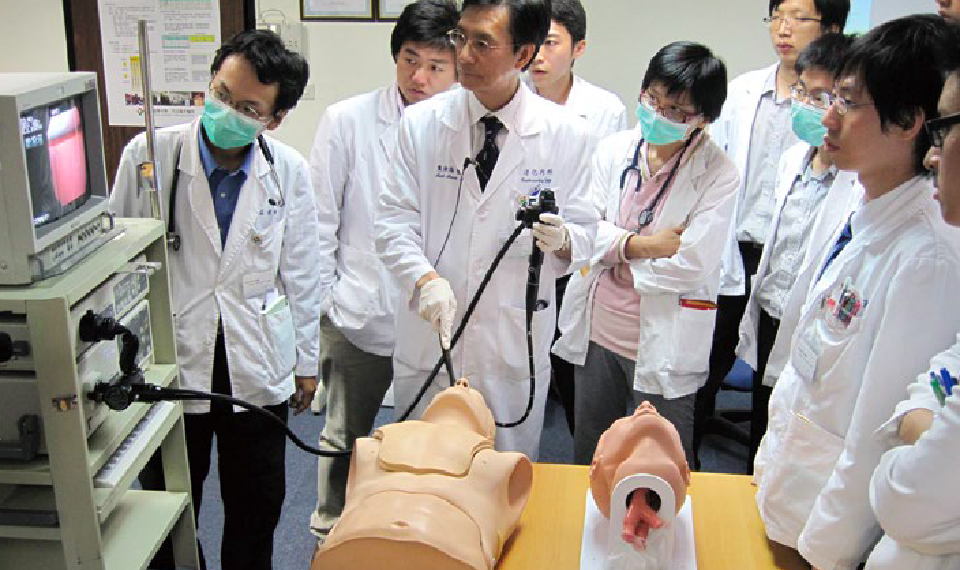
\includegraphics{TMWH_scope.pdf}


%*** using zong Kai Chinese font by \ZongKai{}, and adjust image size \scalebox{h}[v]{}
% image and character: \resizebox{2.7cm}{1.5cm}{}
\ZongKai{\fontsize{3.3}{6}\selectfont \scalebox{1.3}[1.0]{\includesvg[height=1.5cm, distort=false]{TRO_Somaliland.svg}}}
\includesvg[height=1.5cm]{TMWH_logo_TAIPEI_vector.svg}
%\includesvg[height=25.0cm, distort=false]{TRO_Somaliland_font_ZongKai.svg.svg}\hspace{1cm} % TRO logo with ZongKai font in path
\includesvg[height=1.5cm, distort=false]{TMM_logo.svg}
%{2023TMM_officePlate_pink.svg}
\includesvg[height=1.5cm, distort=false]{Hargeisa_Group_Hospital_logo.svg}
%\includesvg[height=1.5cm, distort=false]{MoHD_Somaliland.svg} % 2020
\includesvg[height=1.5cm, distort=false]{logo_MoHD_HGH.svg} 
%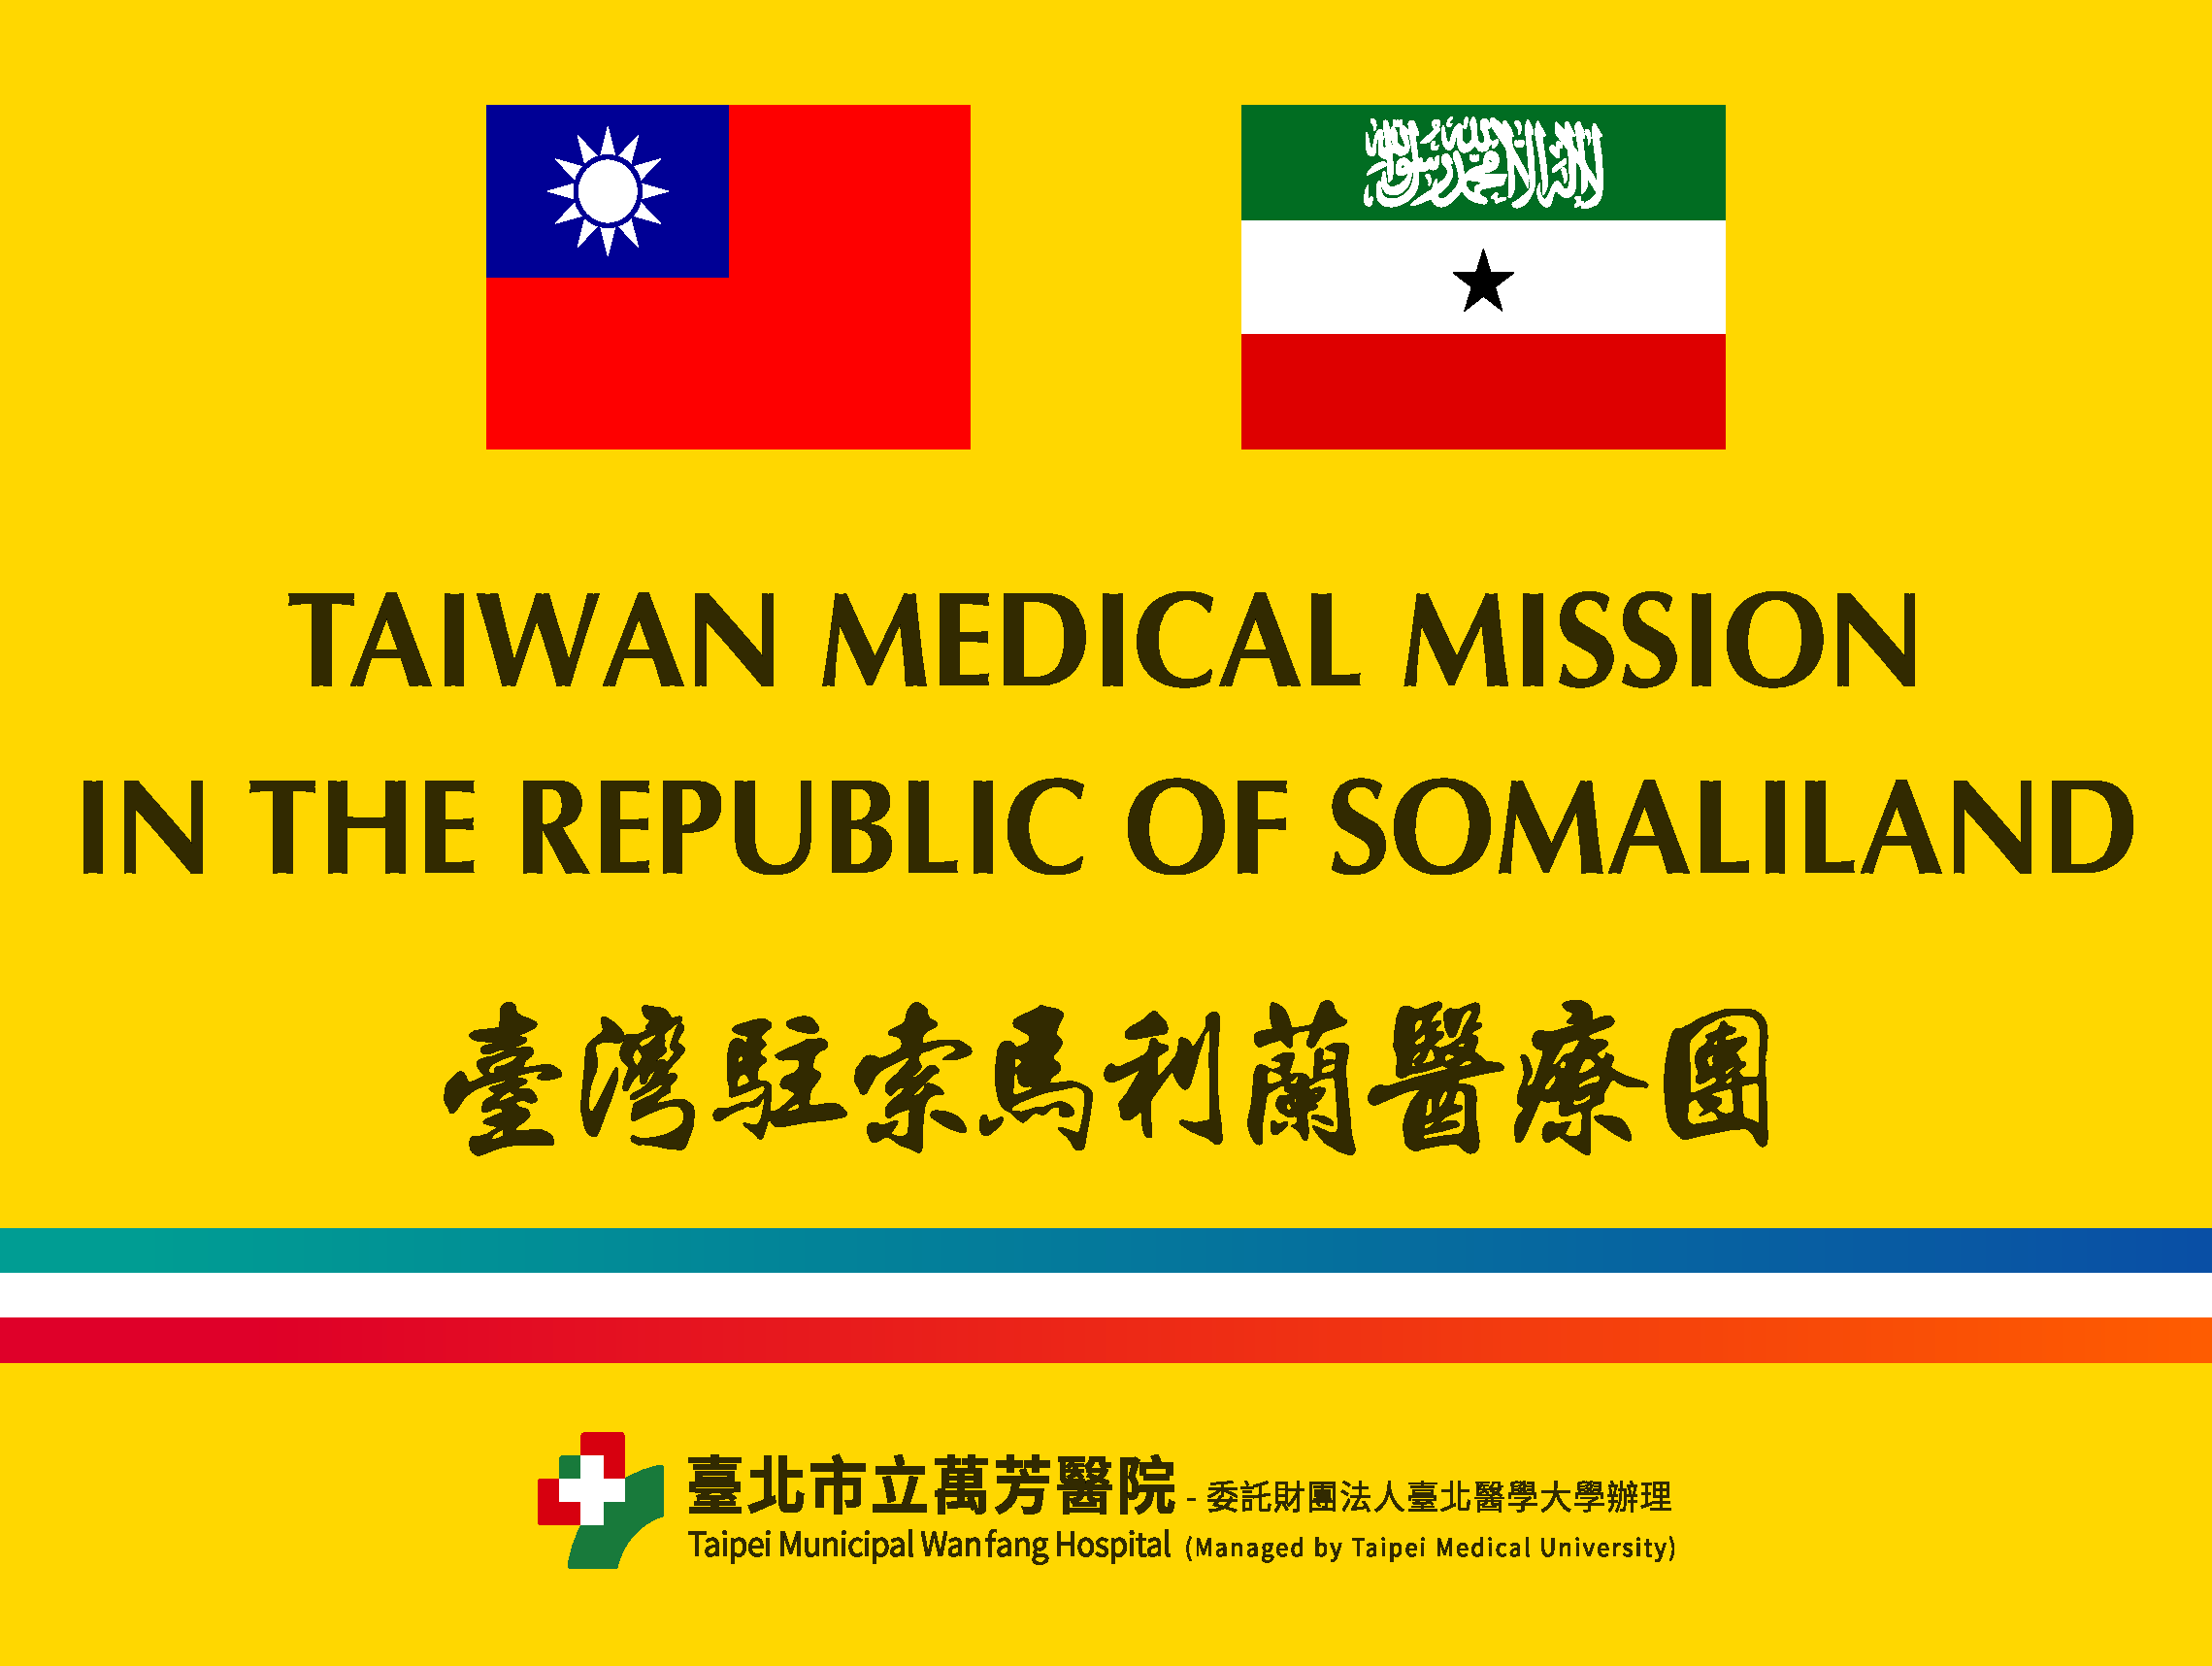
\includegraphics[height=12.0cm, distort=false]{2023TMM_officePlate_ai.pdf}

%%% *********
% ?? add logo of military and social welfare ??

\end{tikzfigure}



%}; % end of node

%} % end of block
